\documentclass{VUMIFPSbakalaurinis}
\usepackage{algorithmicx}
\usepackage{algorithm}
\usepackage{algpseudocode}
\usepackage{amsfonts}
\usepackage{amsmath}
\usepackage{bm}
\usepackage{caption}
\usepackage{color}
\usepackage{float}
\usepackage{graphicx}
\usepackage{listings}
\usepackage{subfig}
\usepackage{wrapfig}

% Titulinio aprašas
\university{Vilniaus universitetas}
\faculty{Matematikos ir informatikos fakultetas}
\department{Programų sistemų katedra}
\papertype{Bakalauro darbas}
\title{-}
\titleineng{-}
\status{4 kurso 5 grupės studentas}
\author{Džiugas Baltramėnas}
\supervisor{asist. Karolis Uosis}
\date{Vilnius – \the\year}

% Nustatymai
%\setmainfont{Time}   % Pakeisti teksto šriftą į Palemonas (turi būti įdiegtas sistemoje)
\bibliography{bibliografija}

\begin{document}
\maketitle

\tableofcontents

\sectionnonum{Įvadas}
    -

    \textbf{Temos aktualumas}: -

    \textbf{Darbo tikslas}:
    -
    \textbf{Darbo Uždaviniai}:
    \begin{enumerate}
        \item -;
        \item -;
        \item -;
        \item -.
    \end{enumerate}

\section{Stacionarus gydymas}

Stacionarus gydymas, arba gydymas stacionare - tai asmens sveikatos priežiūros paslaugos. Šios paslaugos yra teikiamos sveikatos priežiūros įstaigose. Jeigu paslaugų teikimo laikas yra trumpesnis nei para, šios paslaugos yra vadinamos dienos gydymas stacionare, todėl stacionariu gydymu laikoma tokios paslaugos, kurių teikimo laikas yra ilgesnis nei para. Stacionarių paslaugų sąrašą yra patvirtinusi Sveikatos apsaugos ministerija, šį sąrašą sudaro apie 180 paslaugų \cite{StacionaroPaslaugos}. Stacionaraus gydymo paslaugos yra skirstomos į 4 grupes \cite{LigoniuKasa}: 
\begin{itemize}
    \item \textbf{Ilgalaikio gydymo paslaugos} – šios paslaugos teikiamos pacientams, kuriems yra paskirtas ilgo laikotarpio gydymas. Dažniausiai šios paslaugos teikiamos lėtinėmis ligomis sergantiems pacientams.
    \item \textbf{Transplantacijos paslaugos} – šios paslaugos teikiamos pacientams, kuriems reikalingi organų persodinimai. Į šią paslaugų grupę yra įtraukiamos tokios transplantacijos, kaip širdies, plaučių, inkstų, kaulų čiulpų ir kt. 
    \item \textbf{Aktyviojo gydymo paslaugos} – šios paslaugos teikiamos pacientams, kuriems pasireiškė lėtinių lygų pablogėjimas, atsirado agresyvios ligų formos ar patyrė sunkius sužalojimus. Teikiant šį gydymą, pacientas yra ištiriamas, jam skiriami vaistiniai preparatai, teikiamos chirurginės paslaugos, kurios nėra teikiamos ambulatoriniame gydyme.
    \item \textbf{Medicininės reabilitacijos paslaugos} – šios paslaugos teikiamos pacientams, kuriems po sunkių būklių ar susirgimų yra būtina reabilitacija. Sunkių būklių ir susirgimų sąrašą yra patvirtintinus Lietuvos Respublikos sveikatos apsaugos ministerijos.  Šią paslaugų grupę sudaro gydymas vaistiniai preparatais, gydymo dieta, fizioterapijos ir kt.
\end{itemize}

\subsection{Stacionaraus gydymo situacija Lietuvoje}

Tam, kad išsiaiškinti dabartinę Lietuvos stacionaraus gydymo situaciją, autorius pasirinko išnagrinėti stacionaraus gydymo procesus trijose Lietuvos sveikatos priežiūros įstaigose. Pagal Lietuvos statistikos departamento pateiktus duomenis \cite{Gyvento2017}, Jonavos rajono gyventojų tankis yra panašus Lietuvos vidurkiui, todėl buvo pasirinkta nagrinėti Jonavos ligoninė. Nagrinėjant šią ligoninę, buvo laikomasi nuomonės, kad šios ligoninės stacionaraus gydymo procesai bus bendriniai visų rajonų ligoninėms, išskyrus tuos rajonus, kurių gyventojų tankių rodiklius galime laikyti ekstremizmais. Prieš pradedant analizuoti stacionaraus gydymo procesus, autoriui nebuvo žinoma ar karo ligoninėse laikomasi tokių pačių procesų kaip ir civilinėse sveikatos priežiūros įstaigose, todėl buvo pasirinkta nagrinėti vieną iš kariuomenės medicinos punktų, esančios Rukloje. Tam, kad išsiaiškinti ar egzistuoja šių procesų kritiniai skirtumai tarp mažesnių miestelių ligoninių ir didelių, buvo pasirinkta išnagrinėti vieną iš sostinės sveikatos priežiūros įstaigų - Vilniaus universiteto ligoninės Žalgirio klinika. Svarbu pažymėti, kad ne į visas sveikatos priežiūros įstaigas galima patekti asmenims, kurie neturi leidimo, todėl autorius pasirinkto, bendraujant su šių įstaigų darbuotojais, nagrinėti stacionaraus gydymo procesus ir identifikuoti šių procesų gerinimo būdus.

Nors ir aukščiau išvardintos stacionaraus gydymo paslaugų grupės skiriasi viena nuo kitos, tačiau bendrinės procedūros išlieka vienodos. Bendrinėmis stacionaraus gydymo paslaugų procedūromis galime laikyti \cite{Gautam}: 
\begin{itemize}
    \item Medikamentų suteikimas;
    \item Kūno temperatūros matavimas;
    \item Kraujospūdžio ir širdies ritmo matavimas;
    \item Medicininių tyrimų atlikimas;  
\end{itemize}
Šios procedūros yra aptinkamos visose 4 stacionaraus gydymo paslaugų grupėse, tačiau egzistuoja ne tik bendrinės procedūros, bet ir bendrinė stacionaraus gydymo eiga:
\begin{itemize}
    \item [1.] Paciento priėmimas ir lovos suteikimas;
    \item [2.] Paciento gydymo plano sudarymas;
    \item [3-5.] Paciento būklės stebėjimas, medikamentų suteikimas;
    \item [4.] Paskirtiems medicininiams tyrimams, paciento mėginių paėmimas ir tyrimų atlikimas;
    \item [5.] Paskirtų medicininių procedūrų atlikimas;
    \item [6.] Paciento išrašymas.
\end{itemize}

Prieš paguldant pacientą, reikalingas gydymo planas, kuris yra pateikiamas paskyrimo lapo forma. Ši forma užpildoma ir patvirtinama kvalifikuoto gydytojo. Svarbu paminėti tai, jog šis planas gali būti koreguojamas paciento gydymo metu. Plane yra nurodomos reikalingos gydymo procedūros, reikalingos stebėsenos priemonės ir šių priemonių dažnumas, taip pat reikalingi medikamentai ir jų vartojimo dažnumas. Vykdant gydymo planą, kiekviena sąveika su pacientu, kuri yra nurodyta gydymo plane, yra dokumentuojama ir identifikuojamas planą vykdantis darbuotojas.
% (Parasyti apie stebejimo lapa (ar tik gydytojas ji pildo)).
\subsection{Problemos stacionariame gydyme}
2015 metais nacionaliniu mastu buvo įdiegta sveikatos priežiūros informacinė sistema, kuri leidžia visoms sveikatos priežiūros įstaigoms, taip pat ir toms, kurios neturi nuosavų informacinių sistemų, sudaryti gydymo planą bei stebėjimo lapą skaitmenizuotomis formomis, tačiau bendraujant su sveikatos priežiūros įstaigų darbuotojais paaiškėjo, jog dažnu atveju skaitmenizuotos formos nėra naudojamos arba naudojamos kaip antraeilis formų pildymas. Tokios situacijos priežastis - tiriamose įstaigose ši informacinė sistema (arba nuosava įstaigos informacinė sistema) nėra pilnai sudiegta arba jos posistemė, kuri yra skirta aptariamam gydymui, nėra patogi ir intuityvi naudojimui, todėl gydytojui ar slaugytojos darbuotojui patogiau užpildyti dokumentus ranka, o atsiradus laisvai minutei, perkelti dokumentus į skaitmenitizuotą variantą. Atlikus suinteresuotos grupės apklausą, buvo pastebėta, jog skirtingų įstaigų darbuotojai susiduria su bendromis problemomis. Problemos, kurios buvo identifikuotos apklausos metu: 
\begin{itemize}
    \item Laiko eikvojimas perkeliant dokumentus į informacinę sistemą;
    \item Ilgas medikamentų paruošimo vartojimui laikas;
    \item Daug laiko sugaištama pildant popierines formas, kurios reikalingos paciento gydymo formalizavimui.
\end{itemize}

Plačiau apžvelkime identifikuotas problemas:
\begin{itemize}
    \item \textbf{Duomenų perkėlimas}. Nors ir nuo 2015 metų visos sveikatos priežiūros įstaigos gavo prieigą prie nacionaliniu mastu įdiegtos sveikatos priežiūros informacinės sistemos, tačiau naujos technologijos tik padidino sveikatos įstaigų darbuotojų darbo kiekį. Įdiegus šią sistemą, visos sveikatos priežiūros įstaigos buvo įpareigotos teikti skaitmeninius duomenis. Visi darbuotojai dalyvavę apklausose dirba sveikatos priežiūros įstaigose, kurios turi vidinę sistemą, todėl jie neprivalo naudotis nacionaline sistema, nes vidinė sistema komunikuoja su nacionaline, tačiau keletas respondentų yra bandę naudotis nacionaline sistema. Visi respondentai turi panašią nuomonę - nei nacionalinė sistema, nei vidinės sistemos nėra patogios naudojimui. Respondentų nuomone, dokumentų pildymo procedūra greičiau ir efektyviau vyksta tuomet, kai viskas dokumentuojama ranka, o gydymo gale yra perkeliama į skaitmeninį formatą.
    \item \textbf{Medikamentų paruošimo laikas}. Kiekvienam pacientui gydymo plane yra paskiriami medikamentai. Vaistiniai preparatai yra užsakomi griežtai vadovaujantis gydymo planais. Gavus medikamentus stacionaraus gydymo skyriuose, šių skyrių darbuotojai atrūšiuoja medikamentus kiekvienam gydomam pacientui. Atrūšiuoti vaistiniai preparatai yra suteikiami paskirtiems pacientams, tačiau prieš pateikiant juos vartojimui, darbuotojas turi įsitikinti, kad tai išties tas medikamentas, kuris yra paskirtas. Respondentai įvardina jog daugiausiai laiko reikalauja medikamentų rūšiavimas kiekvienam pacientui. Nors respondentai neįvardija medikamentų užsakymo kaip laiko eikvojimo, tačiau, kaip minėta anksčiau, gydymo planai yra pirmiausiai paruošiami popierine forma, o užsakant vaistinius preparatus, medikamentų duomenys yra perkeliami į skaitmeninę formą, t.y. atliekamas dvigubas darbas.
    % ar tikrai perkeliami medikamentai i kompa?
    \item \textbf{Laiko eikvojimas pildant popierines formas}. Ši problema panaši į pirmąją, nors dauguma respondentų mano, kad jiems yra greičiau užpildyti visus reikiamus dokumentus popierine forma, o atsiradus laikui, dokumentus perkelti į sistemą, tačiau pripažįsta, kad popierinių dokumentų pildymas nėra efektyvus ir užima nemažai laiko.
\end{itemize}

Taip pat svarbu pažymėti, jog, apklausos metu, tiek Jonavos ligoninės, tiek Žalgirio klinikos respondentai minėjo susiduriantys su pacientų bandymu įduoti kyšį. Pacientai, kurie bando duoti kyšį, grindžia savo veiksmus tuo, kad darbuotojas, priėmęs kyšį, pacientui suteiks kokybiškesnį gydymą ir priežiūrą, arba bent jau ne prastesnį nei kitiems pacientams. Respondentų minima problema tik patvirtina Valstybinės ligonių kasos darytos apklausos rezultatus \cite{Kasa2016}. Apklausos rezultatai parodė, jog 65\% respondentų mano, jog gydymo ir priežiūros kokybė priklauso nuo kyšio davimo. 

% Nors ši problema nėra klasifikuojama kartu su stacionaraus gydymo procesų problemomis, tačiau šiame darbe bus siūlomi ALR technologija paremti sprendimai, kurie padėtų keisti pacientų nuomonę dėl kyšio davimo ir spręstų išvardintas problemas.





% jei atvyksta i priemima, jis rusiuojamas, pagal sunkuma ligos. Jei su greitaja, tai tiesiai i renimacija. Sutinka sesute ir daktras, ji prima, uzregistruoajam, uzveda forma, iveda i sistema, sumatuoja temp, pulsa, kraujospudi, uzraso kardiograma, priskiria prioriteta ir jis laukia gydytojo apziurojs. Yra formos tam tikros, jas daktaras uzpildo formas, jas atspausdina. Kiekvienas gydytojas palieka savo israsus. 

% Priemime uzveda ligos istorija, joje statusas (pvz: bukle tapati, ar nepablogejus, o jei kazkas atsisitiko skiriami nauji vaistai) turbi buti anspaudas gydytojo. I eina i ta blanka kelios formos, PASKIRIMO lapas, ji uzpildo gydytojas, koreguoja irgi gydytojas, deda parasa. TEn isladinti 3kartus dienoj kazka (laseline, vaistai). Stebejimo lape - statusa nurodo ligonio.

% Dienos stacionare teikiamos nėštumo patologijos, dermatovenerologijos, onkohematologijos, hematologijos, terapijos, vaikų ligų, alerginių ligų, spindulinės terapijos ir kt. paslaugos

% Skaitykite daugiau: https://sveikata.lrytas.lt/sveikas/2016/03/22/news/kas-yra-dienos-stacionaro-paslaugos--1517839/?utm_source=lrExtraLinks&utm_campaign=Copy&utm_medium=Copy

\section{Informacinių technologijų taikymas sveikatos priežiūros įstaigose}
 Kadangi Europos sąjungos populiacija sensta, specialistų nebe užtenka, vadinasi reikalingas sveikatos priežiūrios procesų efektyvumo didėjimas tam, kad padengtų populiacijos reikmes. Šių procesų efektyvumą galime didinti informacinių technologijų pagalba. Toliau šiame skyriuje apžvelgsime informacinių technologijų taikymą Lietuvos sveikatos priežiūros įstaigose.

\subsection{Gydymo įstaigų informacinės sistemos}
Gydymo įstaigų informacinė sistema, kitaip dar vadinama hospitalinė informacinė sistema (toliau - HIS), yra autonominė sveikatos priežiūros įstaigos sistema, kuri orientuojasi į šias veiklas - pacientų registravimas, priėmimas, išleidimas, perkėlimas, apmokestinimas ir kitos administracinės, finansinės ir medicininės funkcijos \cite{Sabooniha2012}. Tam, kad ši sistema išties gerintų sveikatos priežiūros procesų efektyvumą, reikalingas tinkamas duomenų paskirstymas tarp sveikatos priežiūros įstaigos skyrių, todėl šios sistemos pagrindinis uždavinys - apjungti visų skyrių informacines sistemas. Pati HIS nėra laikoma individualaus skyriaus informacine sistema \cite{JuliusGriskevicius}, ji priima klinikinius duomenis iš įstaigos skyrių informacinių sistemų ir juos saugo. Sveikatos priežiūros įstaigos specialistams prireikus pacientų klinikinių duomenų, HIS suteikia prieigą prie jų. Pagrindinės savybės apibūdinančios HIS \cite{JuliusGriskevicius}: 
\begin{enumerate}
    \item Informacijos apie pacientus duomenų bazės;
    \item Pacientų priėmimas ir lovų užimtumo kontrolė;
    \item Analizavimo įrankiai, kurie palengvina sprendimo priėmimą;
    \item Pacientų valdymas ir jų sveikatos įvertinimas;
\end{enumerate}


Tam, kad suprasti Lietuvos sveikatos priežiūros įstaigų naudojamų informacinių sistemų savybes ir funkcionalumus, autorius pasirinko išanalizuoti trijų sveikatos įstaigų HIS. Buvo pasirinkta Kauno regiono asmens sveikatos priežiūros įstaigų HIS (toliau - KRASPI), nes šią HIS naudoja Jonavos ligoninė, ir Vilniaus universiteto ligoninės Žalgirio klinikos HIS (toliau - VULZK HIS). Šios dvi HIS buvo pasirinktos todėl, nes įstaigos, naudojančios šias HIS, buvo pasirinktos stacionaraus gydymo nagrinėjimui ankstesniame skyriuje. Taip pat buvo pasirinkta nagrinėti Vilniaus universiteto ligoninės Santaros klinikos HIS (toliau - VULSK HIS), nes tai yra viena iš didžiausių Lietuvos sveikatos priežiūros įstaigų. Išanalizavimus šių įstaigų HIS specifikacijas, buvo sudaryti palyginimo lentelė (žiūrėti 1 lentelę). 

\begin{table}[!ht]
    \centering
    \renewcommand{\arraystretch}{1.2}
    \begin{tabular}{| p{8em} | c | c | c |}\hline
        \backslashbox[8em]{Savybės}{Įstaigos}
        &\makebox[8em]{KRASPI}&\makebox[8em]{VULZK HIS}&\makebox[8em]{VULSK HIS}\\\hline
        Duomenų centralizuotas kaupimas &+ &+ &+\\\hline
        Pacientų valdymas &+ &+ &+\\\hline
        Duomenų analizavimo įrankiai &- &- &+\\\hline
        Pacientų sveikatos vertinimas &+ &+ &+\\\hline
        Finansinių dokumentų paruošimas &- &+ &+\\\hline
        Lovų užimtumo kontrolė &+ &+ &+\\\hline
    \end{tabular}
    \caption{Sveikatos priežiūros įstaigų informacinių sistemų palyginimas}
    \label{HIS}
\end{table}

Atlikus palyginimą, buvo išsiaiškinta, kad visos nagrinėjamos HIS pasižymi panašiomis savybės ir sprendžia bendras problemas, tačiau tiek Jonavos ligoninės naudojamame HIS, tiek Žalgirio klinikos HIS, trūksta duomenų analizavimo įrankių, taip pat KRASPI nėra finansinių dokumentų paruošimo funkcionalumo.

% &\makebox[8em]{Kauno regiono asmens sveikatos priežiūros įstaigų}&\makebox[8em]{Vilniaus universiteto ligonin4s Santariškių klinikos}&\makebox[8em]{Vilniaus universiteto ligoninės Žalgirio klinika}\\\hline

\subsection{Elektroninė sveikatos paslaugų ir bendradarbiavimo infrastruktūros informacinė sistema}
\subsubsection{Sistemos apžvalga}
Ankstesniame poskyryje apžvelgėme gydymo įstaigų informacines sistemas, tačiau pacientams ne visada sveikatos priežiūros paslaugos teikiamos vienoje gydymo įstaigoje. Pacientui keičiant gydymo įstaigą, iškyla problema - klinikinių paciento duomenų perkėlimas. Šia problemą išsprendžia visos Lietuvos mastu naudojama elektroninė sveikatos paslaugų ir bendradarbiavimo infrastruktūros informacinė sistema (toliau - ESPBI IS). ESPBI IS yra apibrėžiama kaip priemonių visuma, kuri skirta centralizuotai kaupti, formuoti ir naudoti pacientų sveikatos istorijas \cite{ESPBINuostatos}. Šios sistemos dėka, įstaigos, kurios turi prieigos teises, gali tarpusavyje keistis pacientų informacija. Lietuvoje ESPBI IS buvo diegiama 3 etapais, diegimo datos pradžia - 2007 metai, o pabaiga - 2015 metai \cite{Ministras2015}. Kadangi ESPBI IS yra didelės apimties projektas, kuris truko beveik dešimtmetį, dalykinės srities reikalavimai buvo klasifikuojami ir kuriami mažesni projektai šiems reikalavimams įgyvendinti. Pagrindiniai ESPBI IS projektai \cite{Specifikacija}:
\begin{enumerate}
    \item \textbf{Elektroninės sveikatos paslaugų ir bendradarbiavimo infrastruktūra}.
    
    Šio projekto metu sukurtos sistemos pagrindinis funkcionalumas:
    \begin{enumerate}
        \item Pacientų elektroninio sveikatos įrašo tvarkymas;
        \item Paciento registravimasis arba išsiregistravimasis iš sveiktos priežiūros įstaigoje;
        \item Sąveika tarp skirtingų sveikatos priežiūros įstaigų informacinių sistemų;
        \item Aktualių paciento duomenų teikimas ir gavimas;
        \item Finansinių ataskaitų tvarkymas;
        \item Elektroninės tapatybės nustatymas.
    \end{enumerate}
    \item \textbf{Elektroninis receptas}. 
    
    Šio projekto metu sukurtos sistemos pagrindinis funkcionalumas:
    \begin{enumerate}
        \item Elektroninių receptų ar kompensuojamų medicininės pagalbos priemonių išrašymas;
        \item Centralizuotas išrašytų receptų registravimas;
        \item Elektroninių receptų informacijos pateikimas pacientams.
    \end{enumerate}

    \item \textbf{MedVAIS}.
    
    Šio projekto metu sukurtos sistemos pagrindinis funkcionalumas:
    \begin{enumerate}
        \item Sveikatos priežiūros įstaigų sukurtų medicininių vaizdų tvarkymas medicininių vaizdų tvarkymo posistemėje;
        \item Medicininių vaizdų pateikimas pacientams;
        \item Medicininių vaizdų pateikimas gydytojams;
        \item Nuasmeninto medicininio vaizdo pateikimas;
    \end{enumerate}
\end{enumerate}

Kadangi autoriaus projektuojama sistema nėra susijusi nei su medicininiais vaizdai, nei su elektroniniais receptais, tolimesniame nagrinėjime autorius didesnį dėmesį skiria pirmojo projekto analizavimui, o sekantiems dviem projektams dėmesys skiriamas mažesnis.


ESPBI IS paskirtis yra išskiriama į paciento ir sveikatinimo įstaigų atžvilgius \cite{Specifikacija}. Paciento atžvilgiu ESPBI IS paskirtis yra:
\begin{itemize}
    \item Gerinti sveikatingumo paslaugų prieinamumą ir tęstinumą;
    \item Turėti prieigą prie sveikatą apibūdinančių dokumentų;
    \item Plėtoti elektroninės sveikatos paslaugas ir užtikrinti, kad pacientai būtų tinkamai informuojami apie teikiamas paslaugas.
\end{itemize}


Sveikatinimo įstaigų atžvilgiu ESPBI IS paskirtis yra:
\begin{itemize}
    \item Pašalinti paciento duomenų dubliavimą;
    \item Užtikrinant administracinio darbo efektyvumą;
    \item Plėtoti elektroninės sveikatos paslaugas ir užtikrinti, kad įstaigos bendradarbiautų ir gautų aktualią paciento informaciją;
    \item Užtikrinti elektroninės sveikatos paslaugų efektyvumą;
    \item Užtikrinti prieigą prie centralizuotos informacijos.
\end{itemize}

Apibendrinant išvardintas šios sistemos paskirtis, galima teigti, kad siekiama, jog pacientas turėtų galimybę peržiūrėti savo sveikatos istoriją elektroniniu būdų, o įstaigos, efektyviai keistųsi paciento informacija ir ją naudotų tam, kad paslaugų kokybė gerėtų.

\subsubsection{Sistemos architektūra}

Pagal ESPBI IS specifikaciją \cite{Specifikacija} autorius parengė abstrakčią ESPBI IS architektūros diagramą (žiūrėti 1 pav.). 

\begin{figure}[H]
    \centering
    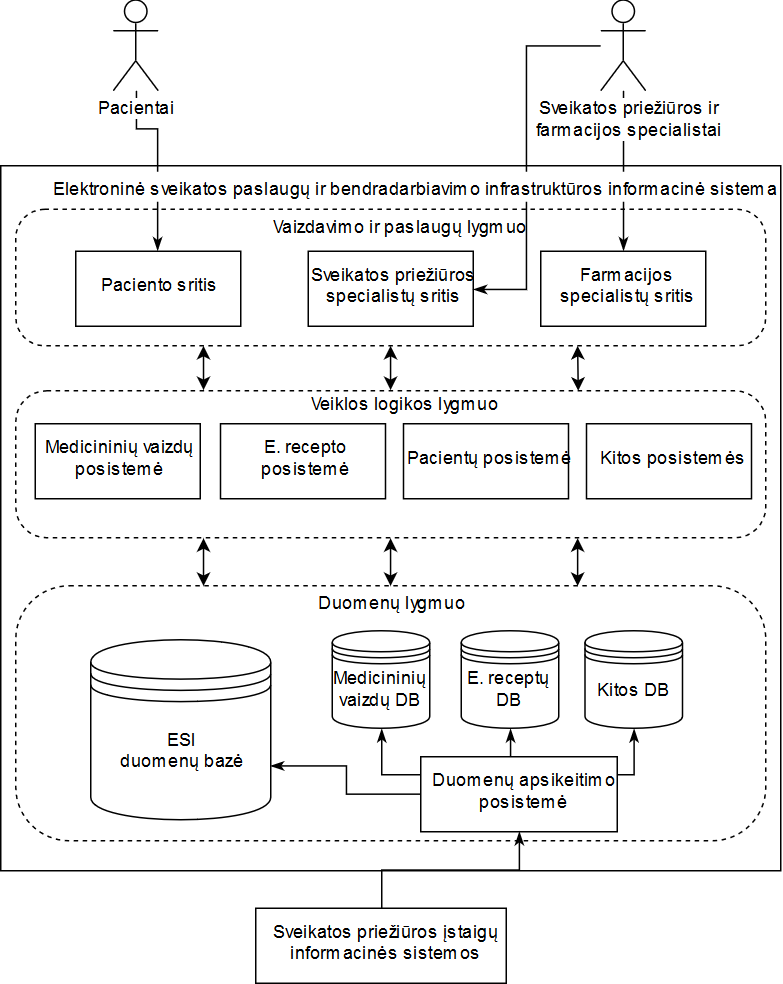
\includegraphics[scale=0.45]{images/ESPBI}
    \caption{Elektroninės sveikatos paslaugų ir bendradarbiavimo infrastruktūros informacinės sistemos achitektūra} 
\end{figure}
% perpiesti, reikia prideti esi posisteme


Pagal parengtos architektūros diagramą matome, kad architektūra yra 3 lygmenų - vaizdavimo ir paslaugų, veiklos logikos ir duomenų lygmens. Išnagrinėkime šiuos tris lygmenis: 

\begin{itemize}
    \item \textbf{Vaizdavimo ir paslaugų lygmuo}. Šį lygmenį sudaro elektroninės sveikatos portalo posistemė. Šio portalo paskirtis - medicininių  paslaugų inicijavimas, šių paslaugų informavimas, jų vykdymo stebėjimas ir suteiktų paslaugų rezultatų pateikimas\cite{Specifikacija}. Šios sistemos naudotojai yra identifikuojami elektroniniu parašu. Prisijungusiam naudotojui yra pateikiamas turinys pagal identifikavimo metu suteiktas prieigas. Elektroninė sveikatos portalo posistemė susideda iš 4 sričių:
    \begin{enumerate}
        \item Viešai prieinama sritis. Šioje elektroninės sveikatos portalo srityje yra pateikiama visiem prieinama informacija. Tam, kad naudotojas pasiektų šią informaciją, jam savo tapatybės identifikuoti nereikia;
        \item Pacientų sritis. Šioje elektroninės sveikatos portalo srityje yra pateikiama paciento gautų paslaugų informacija, rezultatai, išrašytų elektroninių receptų duomenys ir kt;
        \item Sveikatos priežiūros specialistų sritis. Šioje elektroninės sveikatos portalo srityje sveikatos priežiūros specialistai gali pildyti elektroninės sveikatos priežiūros formas, tvarkyti pacientų duomenis, gauti aktualius paciento klinikinius duomenis, medicininius vaizdus, taip pat specialistas, turintis reikiamą prieiga, gali išrašyti pacientui elektroninį receptą, pratęsti jo galiojimo terminą.
        \item Farmacijos specialistų sritis. Ši elektroninės sveikatos portalo sritis yra skirta farmacijos specialistams. Ji leidžia naudotojams  gauti informaciją apie išrašytą elektroninį receptą ir patvirtinti vaistų ar medicininių pagalbos priemonių išdavimo faktą.
    \end{enumerate}
    \item \textbf{Veiklos logikos lygmuo}. Šis lygmuo yra tarpinis tarp vaizdavimo ir duomenų lygmenų.  Veiklos logikos lygmens pagrindinė paskirtis yra priimti sisteminius pranešimus, juos apdoroti, sugeneruoti reikiamą informaciją ir šią informaciją pateikti vaizdavimo ir paslaugų lygmeniui \cite{Specifikacija}. Taip pat šis lygmuo priima duomenis iš elektroninio sveikatos portalo, šiuos duomenis apdoroja ir perduoda į duomenų lygmenį. Apibendrinant šio lygmens paskirtį - tai centrinis funkcionalumų lygmuo, kuris apdoroja ir pateikia reikalingus duomenis apie pacientą, elektroninius receptus, medicininius vaizdus ir kt. Šį lygmenį sudaro 11 posistemių, tačiau pagrindinės yra: 
    \begin{enumerate}
        \item Pacientų posistemė;
        \item Medicininių  vaizdų posistemė;
        \item Elektroninio recepto posistemė;
        \item Duomenų analizės, ataskaitų formavimo ir informavimo posistemė;
        \item Elektroninio sveikatos įrašo posistemė.
    \end{enumerate}
    \item \textbf{Duomenų lygmuo}. Duomenų lygmuo susideda iš 2 komponentų - informacinės struktūros ir duomenų mainų posistemės. Apžvelkime šiuos komponentus:
    \begin{itemize}
        \item Informacinė struktūra. Šis komponentas atsakingas už ESPBI IS informacijos tvarkymą, saugojimą, apdorojimą ir teikimą. Pagrindinis informacinės struktūros komponentas yra ESI duomenų bazė, tačiau informacinė struktūrą sudaro ir daugiau papildomų duomenų bazių \cite{Specifikacija}, iš viso yra 10 duomenų bazių, kurios saugo informaciją apie sveikatos priežiūros paslaugų teikimą. ESI duomenų bazėje saugomi pacientų elektroniniai sveikatos įrašai, kurie yra suvedami paslaugų ir vaizdavimo lygmenyje arba gaunami iš sveikatos priežiūros įstaigų informacinių sistemų. Kiekvienas įrašas yra susiejimas su identifikatoriumi, kuris yra suteikiamas Objektų ID katalogo. Objektų ID katalogas suteiktą identifikatorių susieja su paciento įrašu, specialistu, kuris pateikė paciento įrašą, ir sveikatos priežiūros įstaiga. ESI duomenų bazės tvarkomi dokumentai \cite{Specifikacija}: ypatingieji pacientų duomenys, ESI suformavusių sveikatinimo specialistų duomenys, ESI pateikusių sveikatinimo įstaigų duomenys;
        \item Duomenų mainų posistemė. Šis komponentas atsakingas už duomenų priėmimą bei atidavimą sveikatos priežiūros įstaigų informacinėms sistemoms bei kitoms suinteresuotų trečiųjų šalių informacinėms sistemos. Ši posistemė yra kertinis komponentas, kuris realizuoja techninio interoperabilumo principus elektroninės sveikatos sistemoje \cite{Specifikacija}. Duomenų mainų posistemės pagrindinė paskirtis - valdyti duomenų mainus tarp sveikatos priežiūros įstaigų ir užtikrinti duomenų gavimą bei teikimą tokioms įstaigom kaip SODRA, SVEIDRA, VAPRIS ir kitomis valstybinėms institucijom. Visi duomenų mainai tarp ESPBI IS ir kitų informacinių sistemų vyksta per šią posistemę.
    \end{itemize}
\end{itemize}

\subsubsection{Septinto lygio sveikatos standartas}
Ankstesniuose poskyriuose apžvelgėme Lietuvos sveikatos priežiūros įstaigų naudojamas informacines sistemas, tačiau Lietuva nėra išskirtinė šioje srityje ir kitos Europos sąjungos valstybės taip pat diegia bei naudoja tokio pat pobūdžio informacines sistemas, šių sistemų diegimo bei naudojimo būsena yra aprašyta Europos Komisijos \cite{EuroposKomisija}. Europos parlamento priimtose direktyvose \cite{EuroposParlamentas} yra nurodoma, jog valstybės turi tarpusavyje dalintis pacientų sveikatos įrašais, t.y. pacientui apsilankius svetimos valstybės sveikatos priežiūros įstaigoje, ši įstaiga galėtų gauti paciento duomenis iš jo gimtosios valstybės. Kadangi siekiama pacientų duomenų keitimosi ne tik regioniniu mastu, bet ir tarpvalstybiniu, vadinasi visos tarpusavyje komunikuojančios informacinės sistemos turi vadovautis bendru tarptautiniu standartu, kuris aprašytų pacientų duomenų apsikeitimo procesą. Toks pacientų duomenų apsikeitimo standartas yra Septintojo lygio sveikatos standartas (angl. \textit{Health Level Seven International}) (toliau - HL7). HL7 standartas, kurio pirmoji versija buvo sukurta 1987 metais, yra patvirtintas Amerikos nacionalinio standartų instituto, šis standartas apibrėžia elektroninių sveikatos įrašų paiešką, dalijimąsi, integraciją ir apsikeitimą \cite{HL72009}. HL7 nusako kaip įstaigos keičiasi elektroniniais sveikatos įrašais ir kokiu duomenų formatu šie įrašai yra suformuoti. HL7 yra apibrėžęs 2 duomenų formatus - v2 ir v3, taip pat egzistuoja ir FHIR standartas, kuris apjungia labiausiai pasiteisinusius HL7 v2 ir v3 standartų aspektus. ESPBI IS specifikacijoje \cite{Specifikacija} yra nurodoma, jog duomenų apsikeitimui yra naudojamas HL7 v3 arba FHIR standartai, tačiau naujesnėje literatūroje \cite{Registrucentras} yra nurodomas tik FHIR. FHIR standartas apibrėžia netik duomenų formavimą, bet ir pateikia REST architektūra pagrįstą interfeisą, kuris nurodo
% paaiskint interfeisa ir resta, crud
duomenų operacijoms reikalingus CRUD metodus.


% issiaiskinti del ruklos, kam ji priklauso ( Jei priklauso kazkam is saraso, galim prideti saltini prie hospitalisation.tex)
% neiasku del duomenu baziu, lape raso, kad ji viena yra, o realiai ju daug


\subsection{Stacionariame gydyme pasitaikančių problemų sprendimo būdai}

Su stacionaraus gydymo problemomis, kurios buvo identifikuotos pirmąjame skyriuje, yra susiduriama ne tik Lietuvoje. Jungtinėse Amerikos Valstijose pradėjus sveikatos įstaigose diegti informacines sistemas, atsirado daug problemų, kurios trukdė šių sistemų diegimui bei naudojimui. Viena iš problemų - sveikatos įstaigų darbuotojai nemoka naudotis informacinėmis technologijomis \cite{Jha2009}. Ši problema mažina darbuotojų produktyvumą, nes informacinių sistemų naudojimas užima perdaug laiko. Tam, kad sveikatos priežiūros įstaigų darbuotojai gebėtų efektyviai dirbti su naujausiomis technologijomis, labai svarbus yra jų įtraukimas į diegimo procesą, edukavimas ir kompetentingų žmonių pagalba \cite{Lorenzi2009}. Duomenų įvedimo sunkumai taip pat yra sprendžiami šablonų bei automatinio teksto funkcijomis \cite{Noblin2013}. Darbuotojams yra lengviau pildyti dokumentas pagal pateiktus šablonus bei instrukcijas, o automatinio teksto funkcija paspartina duomenų įvedimą į sistemą. 

Taip pat pirmąjame skyriuje buvo identifikuota medikamentų paruošimo problema. Nors daugiausiai laiko paruošimo procese užima medikamentų rūšiavimas kiekvienam pacientui, tačiau šis etapas yra gyvybiškai svarbus, nes suklydus ir pateikus netinkamą vaistą pacientui, pasekmės gali būti kritinės. Medikamentų adiministravimo problemas siūloma spręsti šiais būdais \cite{Agrawal2009}:
\begin{itemize}
    \item Paskirtų medikamentų informaciją skaitmenitizuoti;
    \item Medikamentus sužymėti brūkšninias kodais (angl. \textit{barcode}), kur brūkšniniame kode būtų laikoma paciento, kuriam paskirtas vaistas, informacija;
    \item Medikamentų užsakymo sistema (angl. \textit{Computerized physician order entry, CPOE}). Ši sistema apjungia sveikatos ir farmacijos įstaigas, padeda atlikti medikamentų užsakymus.
\end{itemize}

Pagal pateiktus problemų sprendimo pavyzdžius matome, kad dauguma jų sprendžia duomenų įvedimo problemą. Ši problema taip pat gali būti sprendžiama artimojo lauko ryšio technologija. Pagrindiniai argumentai, kodėl artimojo lauko ryšio technologija gali padėti spręsti minėtas problemas \cite{forum2}: 
\begin{itemize}
    \item Paprastas paciento duomenų perkėlimas;
    \item Užtikrintumas dėl informacijos tikslumo konkrečiam pacientui;
    \item Paprastas įrenginių prilietimas nereikalauja darbuotojų mokymų;
    \item Lengvas pacientui paskirtų medikamentų identifikavimas.
\end{itemize}

\sectionnonum{Rezultatai ir išvados}

Atlikus darbą buvo gauti šie \textbf{rezultatai}:
\begin{enumerate}
    \item -;
    \item -;
    \item -;
    \item -.
\end{enumerate}

Darbo \textbf{išvados}:
\begin{enumerate}
    \item -;
    \item -;
    \item -;
    \item -.
\end{enumerate}

\printbibliography[heading=bibintoc]  % Šaltinių sąraše nurodoma panaudota
% literatūra, kitokie šaltiniai. Abėcėlės tvarka išdėstomi darbe panaudotų
% (cituotų, perfrazuotų ar bent paminėtų) mokslo leidinių, kitokių publikacijų
% bibliografiniai aprašai.  Šaltinių sąrašas spausdinamas iš naujo puslapio.
% Aprašai pateikiami netransliteruoti. Šaltinių sąraše negali būti tokių
% šaltinių, kurie nebuvo paminėti tekste.

\sectionnonum{Sąvokų apibrėžimai}
\begin{enumerate}
    \item -;
    \item -;
    \item -;
    \item -.
\end{enumerate}

\end{document}
